\section{Kiểm thử Hệ thống}

\subsection{Công cụ kiểm thử}

\subsubsection{Google Lighthouse}
Google Lighthouse là một công cụ kiểm thử và phân tích website 
mã nguồn mở do Google phát triển, được sử dụng rộng rãi trong 
việc đánh giá chất lượng và tối ưu hóa trang web \cite{lighthouse_docs}. 
Công cụ này có thể chạy trực tiếp trên Chrome DevTools, cài đặt 
dưới dạng tiện ích mở rộng hoặc sử dụng qua dòng lệnh. Khi thực 
hiện kiểm tra, Lighthouse tự động phân tích nhiều khía cạnh quan 
trọng của website bao gồm hiệu năng tải trang (Performance), khả 
năng truy cập (Accessibility), mức độ tuân thủ các chuẩn SEO, 
các thực hành tốt về bảo mật (Best Practices) và khả năng hỗ trợ 
Progressive Web App (PWA). Sau quá trình đánh giá, công cụ cung 
cấp báo cáo chi tiết kèm các chỉ số Core Web Vitals (FCP, LCP, 
CLS, TBT, Speed Index) và gợi ý cải thiện cụ thể.

\subsubsection{Postman}
Postman là công cụ kiểm thử API phổ biến, cho phép gửi các yêu 
cầu HTTP đến server và kiểm tra phản hồi một cách trực quan 
\cite{postman_docs}. Trong đề tài, Postman được sử dụng để kiểm 
thử các endpoint của FastAPI backend bao gồm xác thực JWT, upload 
ảnh cho AI Virtual Try-On, các API quản lý sản phẩm, đơn hàng, 
chatbot và thanh toán Stripe. Postman hỗ trợ kiểm thử với 
multipart/form-data, thiết lập header xác thực và lưu trữ 
collection test case có tổ chức.

\subsubsection{Swagger UI}
Swagger UI là giao diện tài liệu và kiểm thử API được FastAPI 
tự động sinh ra tại đường dẫn \texttt{/docs} \cite{fastapi_docs}. 
Công cụ này cho phép kiểm thử trực tiếp tất cả endpoint của hệ 
thống ngay trên trình duyệt mà không cần cài đặt thêm phần mềm, 
đồng thời hiển thị đầy đủ schema request và response của từng API.

\subsubsection{Responsive Viewer}
Responsive Viewer là tiện ích mở rộng (extension) của trình duyệt 
Chrome, cho phép kiểm tra giao diện website trên nhiều kích thước 
màn hình cùng lúc \cite{responsive_viewer}. Trong đề tài, công cụ 
này được sử dụng để kiểm thử tính tương thích giao diện của hệ 
thống trên các thiết bị di động, máy tính bảng và máy tính để bàn 
mà không cần thiết bị vật lý.

% ─────────────────────────────────────────
\subsection{Kiểm thử}

\subsubsection{Kiểm thử API}

Các endpoint của hệ thống được kiểm thử thông qua Postman và 
Swagger UI. Bảng~\ref{tab:api_test} trình bày một số test case 
tiêu biểu.

\begin{table}[H]
\centering
\caption{Một số test case kiểm thử API}
\label{tab:api_test}
\begin{tabular}{|c|p{3cm}|p{3cm}|p{3cm}|c|}
\hline
\textbf{STT} & \textbf{Endpoint} & \textbf{Input} & 
\textbf{Kết quả mong đợi} & \textbf{Kết quả} \\
\hline
1 & POST /users & Firebase UID hợp lệ & 
Upsert user thành công, trả về thông tin user & Đạt \\
\hline
2 & GET /garments/ & -- & 
Trả về danh sách garment & Đạt \\
\hline
3 & POST /tryon & Ảnh người + ảnh quần áo & 
Trả về URL ảnh kết quả từ Cloudinary & Đạt \\
\hline
4 & POST /photo-tryon/fit-assessment & 
body\_profile\_id, garment\_id, size\_label & 
Trả về đánh giá chest\_fit, waist\_fit, hip\_fit, 
size\_suggestion & Đạt \\
\hline
5 & POST /chatbot/chat & Câu hỏi tư vấn thời trang & 
Trả về phản hồi từ Ollama qwen2.5 & Đạt \\
\hline
6 & POST /payment/stripe & Thông tin đơn hàng & 
Tạo payment intent thành công & Đạt \\
\hline
7 & POST /tryon & Thiếu file ảnh & 
Trả về lỗi 422 Unprocessable Entity & Đạt \\
\hline
\end{tabular}
\end{table}
\subsubsection{Kết quả thực nghiệm AI Try-On (FitDiT)}

Thực nghiệm đo thời gian xử lý của mô hình FitDiT được thực hiện trên
GPU NVIDIA RTX 4060 Laptop (8GB VRAM) với cùng một cặp ảnh đầu vào
(ảnh người và ảnh quần áo), thay đổi số bước lặp (num\_steps) để đánh
giá ảnh hưởng đến thời gian xử lý. Mỗi mức được đo 2 lần lấy trung bình,
các lần bị timeout do quá tải GPU không được tính vào kết quả.

\begin{table}[H]
\centering
\caption{Kết quả đo thời gian xử lý FitDiT theo số bước lặp}
\label{tab:fitdit_benchmark}
\begin{tabular}{|c|c|c|c|}
\hline
\textbf{num\_steps} & \textbf{Lần 1 (s)} & \textbf{Lần 2 (s)} & \textbf{Trung bình (s)} \\
\hline
10 & 28,00 & 34,44 & 31,22 \\
\hline
20 & 41,68 & 41,53 & 41,61 \\
\hline
\end{tabular}
\end{table}

Kết quả cho thấy khi tăng số bước lặp từ 10 lên 20, thời gian xử lý
tăng khoảng 33\% (từ 31,22 giây lên 41,61 giây). Hệ thống mặc định
sử dụng \textbf{num\_steps = 15} để cân bằng giữa chất lượng ảnh và
thời gian phản hồi. Do giới hạn phần cứng GPU laptop (RTX 4060, 8GB VRAM),
thời gian xử lý chưa đáp ứng được yêu cầu real-time. Hướng cải thiện
là triển khai lên GPU cloud (RunPod, Vast.ai) hoặc tối ưu với TensorRT
để rút ngắn thời gian xuống dưới 10 giây.

\subsubsection{So sánh hai phương pháp thử đồ ảo}

\begin{table}[H]
\centering
\caption{So sánh tổng hợp hai phương pháp thử đồ ảo}
\label{tab:tryon_compare}
\begin{tabular}{|p{3.5cm}|p{4cm}|p{4cm}|}
\hline
\textbf{Tiêu chí} & \textbf{AR Try-On} & \textbf{AI Try-On (FitDiT)} \\
\hline
Thời gian phản hồi & Dưới 1 giây & 31--42 giây (10--20 bước) \\
\hline
Độ chân thực & Trung bình (mô hình 3D) & Cao (Diffusion Transformer) \\
\hline
Độ khớp trang phục & Tốt ở tư thế đứng yên & Rất tốt, theo sát dáng người \\
\hline
Bảo toàn texture & Tốt (nhúng trong 3D model) & Rất tốt (giữ nguyên hoa văn, màu sắc) \\
\hline
Yêu cầu đầu vào & Camera trực tiếp & Ảnh người + ảnh quần áo \\
\hline
Yêu cầu phần cứng & Camera + GPU trình duyệt & GPU server (RTX 4060+) \\
\hline
Tính tương tác & Thời gian thực & Không tương tác \\
\hline
Phù hợp với & Xem nhanh, tương tác tức thì & Xem chi tiết trước khi mua \\
\hline
\end{tabular}
\end{table}

\subsubsection{Nhận xét tổng quan}

Kết quả thực nghiệm cho thấy hai phương pháp bổ trợ lẫn nhau và phù
hợp với các ngữ cảnh sử dụng khác nhau. Phương pháp AR cho phản hồi
tức thì nhưng độ chân thực còn hạn chế do phụ thuộc vào chất lượng
mô hình 3D và điều kiện ánh sáng môi trường. Phương pháp AI FitDiT
cho kết quả chân thực cao hơn đáng kể nhờ Diffusion Transformer tổng
hợp ảnh từ đặc trưng cơ thể và trang phục, tuy nhiên thời gian xử lý
còn chậm do giới hạn phần cứng GPU laptop.

Việc kết hợp cả hai phương pháp trong cùng một hệ thống là lựa chọn
hợp lý: người dùng có thể dùng AR để xem nhanh trang phục ngay trên
trang sản phẩm, sau đó dùng AI Try-On để xem kết quả chi tiết trước
khi quyết định mua hàng. Sự kết hợp này giúp giảm thiểu tỷ lệ hoàn
trả hàng do chọn sai trang phục, đồng thời nâng cao trải nghiệm mua
sắm trực tuyến.
% ─────────────────────────────────────────
\subsubsection{Kiểm thử hiệu năng AR Try-On theo điều kiện chuyển động}

Để đánh giá hiệu năng hiển thị của chức năng AR Try-On trong các điều
kiện sử dụng thực tế, thực nghiệm đo số khung hình mỗi giây (FPS) được
thực hiện trên trình duyệt Google Chrome thông qua script
\texttt{requestAnimationFrame} counter. Mỗi lần đo kéo dài \textbf{30 giây},
lấy mẫu theo từng giây và tính trung bình trên toàn bộ chuỗi mẫu.
Ba điều kiện kiểm thử được thiết lập như sau:

\begin{itemize}
    \item \textbf{Lần 1 -- Đứng yên, ánh sáng tốt:} Camera và người dùng
    giữ nguyên tư thế; điều kiện ánh sáng môi trường ổn định. Đây là
    kịch bản cơ sở (baseline).
    \item \textbf{Lần 2 -- Cử động tay/người chậm:} Người dùng di chuyển
    tay hoặc cơ thể với tốc độ thấp, mô phỏng thao tác tương tác thông thường.
    \item \textbf{Lần 3 -- Cử động tay/người nhanh:} Người dùng di chuyển
    tay hoặc cơ thể với tốc độ cao, mô phỏng chuyển động đột ngột hoặc
    xoay người nhanh.
\end{itemize}

\begin{table}[H]
\centering
\caption{Kết quả đo FPS của AR Try-On theo điều kiện chuyển động}
\label{tab:ar_fps}
\renewcommand{\arraystretch}{1.5}
\begin{tabular}{|c|p{3.8cm}|c|c|c|c|}
\hline
\textbf{Lần} & \textbf{Điều kiện} &
\textbf{$\overline{FPS}$} & \textbf{$FPS_{\min}$} & \textbf{$FPS_{\max}$} &
\textbf{Frame Drop} \\
\hline
1 & Đứng yên, ánh sáng tốt  & 144{,}8 & 144 & 146 & 0 \\
\hline
2 & Cử động tay/người chậm  & 142{,}3 & 108 & 145 & 1 \\
\hline
3 & Cử động tay/người nhanh & 138{,}1 &  50 & 145 & 2 \\
\hline
\end{tabular}
\end{table}

\textit{Ghi chú: Frame Drop được tính là số giây ghi nhận FPS dưới 120\,fps
trong chuỗi 30 mẫu.}

Kết quả cho thấy AR Try-On duy trì hiệu năng rất cao ở điều kiện đứng yên
($\overline{FPS} = 144{,}8$), vượt xa ngưỡng 60\,fps yêu cầu cho trải nghiệm
mượt mà. Khi người dùng cử động chậm, FPS trung bình giảm nhẹ xuống 142{,}3
và xuất hiện một frame drop duy nhất (108\,fps), hệ thống vẫn hoạt động ổn
định. Ở điều kiện cử động nhanh, FPS tối thiểu giảm xuống 50\,fps tại một
số thời điểm do motion blur khiến thuật toán nhận diện đặc trưng mất nhiều
chu kỳ xử lý hơn; tuy nhiên FPS trung bình vẫn đạt 138{,}1\,fps, đảm bảo
trải nghiệm không bị gián đoạn trong phần lớn thời gian sử dụng.
% ─────────────────────────────────────────
\subsubsection{Đánh giá chất lượng ảnh AI Try-On bằng SSIM, PSNR và LPIPS}

Ngoài việc đo thời gian xử lý, đề tài còn đánh giá chất lượng ảnh đầu ra
của mô hình FitDiT thông qua ba chỉ số phổ biến trong lĩnh vực xử lý ảnh:

\begin{itemize}
    \item \textbf{SSIM (Structural Similarity Index):} đo mức độ tương đồng
    về cấu trúc hình ảnh giữa hai ảnh, giá trị nằm trong khoảng $[0,1]$.
    Giá trị càng gần 1 thì ảnh càng giống nhau.

    \item \textbf{PSNR (Peak Signal-to-Noise Ratio):} đo mức độ sai khác
    tín hiệu giữa hai ảnh. Giá trị càng cao thì chất lượng ảnh càng tốt.

    \item \textbf{LPIPS (Learned Perceptual Image Patch Similarity):}
    đo sự khác biệt cảm nhận thị giác bằng deep learning. Giá trị càng thấp
    thì hai ảnh càng giống nhau theo cảm nhận của con người.
\end{itemize}

Thực nghiệm được thực hiện với cùng một ảnh người, cùng một ảnh quần áo,
cùng giá trị \texttt{guidance=2}, cùng \texttt{seed=42} và cùng độ phân giải
\texttt{768$\times$1024}. Chỉ thay đổi số bước lặp (\texttt{num\_steps})
để đánh giá ảnh hưởng đến chất lượng ảnh đầu ra.

Ảnh được sinh với \texttt{num\_steps=20} được chọn làm ảnh chuẩn (baseline)
để so sánh với các mức khác.

\begin{table}[H]
\centering
\caption{So sánh chất lượng ảnh theo số bước lặp}
\label{tab:fitdit_quality}
\renewcommand{\arraystretch}{1.4}
\begin{tabular}{|c|c|c|c|}
\hline
\textbf{So sánh} & \textbf{SSIM} & \textbf{PSNR} & \textbf{LPIPS} \\
\hline
20 bước vs 25 bước & 0.9976 & 48.61 & 0.0002 \\
\hline
20 bước vs 10 bước & 0.7815 & 12.72 & 0.3545 \\
\hline
\end{tabular}
\end{table}

Kết quả cho thấy ảnh sinh với \texttt{25 bước} gần như tương đồng hoàn toàn
so với \texttt{20 bước}, thể hiện qua chỉ số SSIM đạt 0.9976 và LPIPS gần bằng 0.
Điều này cho thấy việc tăng thêm số bước từ 20 lên 25 gần như không cải thiện
đáng kể chất lượng ảnh nhưng lại làm tăng thời gian xử lý.

Ngược lại, ảnh sinh với \texttt{10 bước} có độ khác biệt đáng kể so với
\texttt{20 bước}, thể hiện qua SSIM chỉ đạt khoảng 0.78 và LPIPS tăng lên
0.35. Trong thực tế, ảnh 10 bước xuất hiện nhiều lỗi hơn như mất chi tiết
texture, biến dạng vùng tay áo và giảm độ chân thực tổng thể.

Từ kết quả trên, hệ thống lựa chọn \textbf{num\_steps = 15} làm cấu hình mặc định
để cân bằng giữa chất lượng ảnh và thời gian phản hồi trên phần cứng GPU RTX 4060.

% ─────────────────────────────────────────
\subsubsection{Đánh giá độ chính xác trực quan của AI Try-On}

Ngoài các chỉ số định lượng, đề tài còn thực hiện đánh giá trực quan
để kiểm tra mức độ chính xác của chức năng thử đồ ảo AI Try-On.
Việc đánh giá được thực hiện trên nhiều ảnh người với các tư thế và
trang phục khác nhau nhằm quan sát khả năng:

\begin{itemize}
    \item Giữ đúng hình dạng và tỷ lệ trang phục
    \item Bảo toàn texture, màu sắc và logo trên quần áo
    \item Phù hợp với dáng người và tư thế cơ thể
    \item Hạn chế biến dạng ở vùng tay áo, cổ áo và vai
    \item Đảm bảo tính chân thực tổng thể của ảnh sinh ra
\end{itemize}

\begin{table}[H]
\centering
\caption{Đánh giá trực quan chất lượng AI Try-On}
\label{tab:visual_quality}
\renewcommand{\arraystretch}{1.4}
\begin{tabular}{|p{4cm}|c|p{6cm}|}
\hline
\textbf{Tiêu chí đánh giá} & \textbf{Mức độ} & \textbf{Nhận xét} \\
\hline
Độ khớp trang phục & Tốt &
Trang phục bám sát cơ thể và giữ đúng tỷ lệ tổng thể \\
\hline
Bảo toàn texture & Rất tốt &
Logo, họa tiết và màu sắc được giữ gần giống ảnh gốc \\
\hline
Độ chân thực & Tốt &
Ảnh tạo ra có độ tự nhiên cao trong điều kiện ánh sáng ổn định \\
\hline
Xử lý vùng tay áo & Trung bình &
Một số trường hợp xuất hiện biến dạng nhẹ khi tay che cơ thể \\
\hline
Xử lý tư thế phức tạp & Trung bình &
Giảm chất lượng khi người mẫu xoay người hoặc tạo dáng mạnh \\
\hline
\end{tabular}
\end{table}

Kết quả thực nghiệm cho thấy mô hình FitDiT có khả năng tái tạo
trang phục với độ chân thực cao, đặc biệt ở các tư thế đứng thẳng
và điều kiện ánh sáng ổn định. Texture và màu sắc của quần áo được
bảo toàn tốt trong đa số trường hợp.

Tuy nhiên, một số lỗi vẫn xuất hiện khi người mẫu có tư thế phức tạp
hoặc vùng cánh tay che khuất nhiều phần cơ thể. Các lỗi phổ biến bao gồm:

\begin{itemize}
    \item Biến dạng nhẹ vùng tay áo
    \item Mất chi tiết texture ở vùng bị che khuất
    \item Sai lệch nhỏ tại viền cổ áo hoặc vai áo
\end{itemize}

\begin{figure}[H]
    \centering
    
    % Ảnh người gốc
    \begin{minipage}{0.32\textwidth}
        \centering
        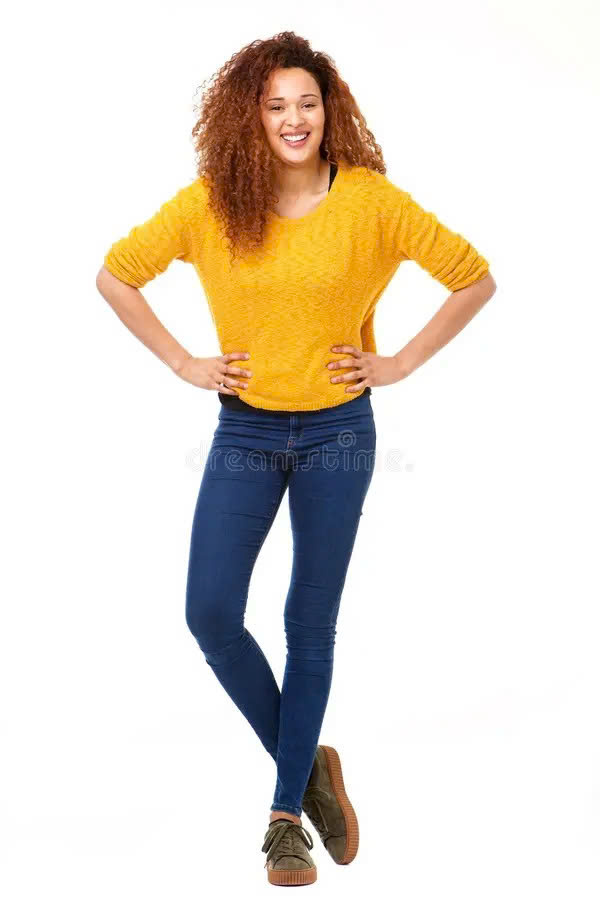
\includegraphics[width=\linewidth]{graphics/main/test/person_input.jpg}
        \caption*{(a) Ảnh người gốc}
    \end{minipage}
    \hfill
    
    % Ảnh quần áo gốc
    \begin{minipage}{0.32\textwidth}
        \centering
        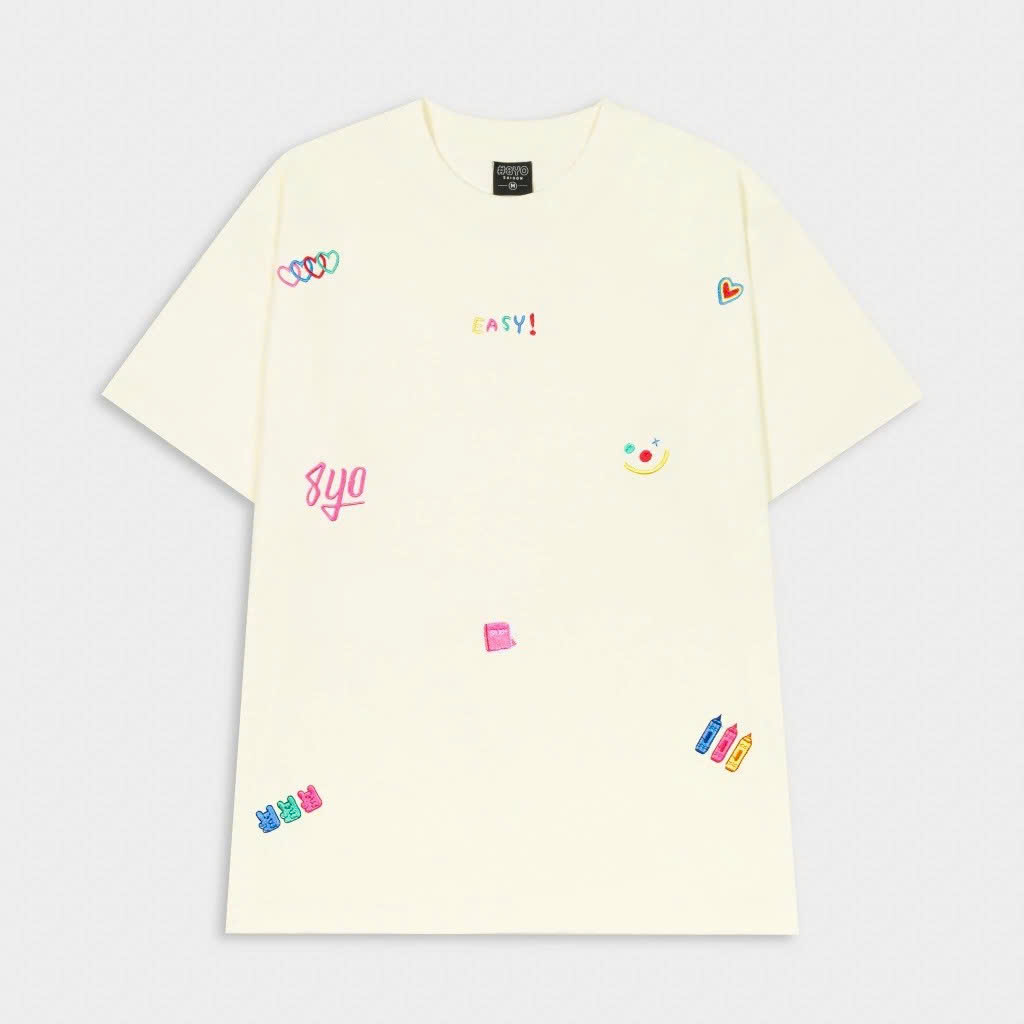
\includegraphics[width=\linewidth]{graphics/main/test/garment_input.jpg}
        \caption*{(b) Ảnh quần áo}
    \end{minipage}
    \hfill
    
    % Kết quả AI Try-On
    \begin{minipage}{0.32\textwidth}
        \centering
        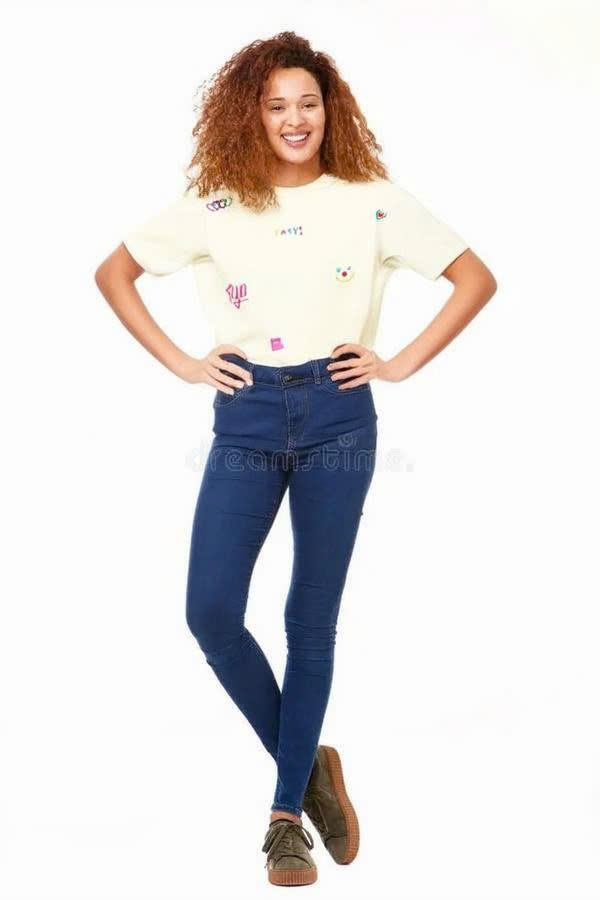
\includegraphics[width=\linewidth]{graphics/main/test/tryon_result.jpg}
        \caption*{(c) Kết quả AI Try-On}
    \end{minipage}
    
    \caption{So sánh ảnh đầu vào và kết quả AI Try-On}
    \label{fig:tryon_compare}
\end{figure}

So với phương pháp AR Try-On sử dụng mô hình 3D, AI Try-On cho kết quả
chân thực hơn đáng kể do ảnh được tổng hợp trực tiếp bằng mô hình
Diffusion Transformer thay vì chỉ phủ texture lên mô hình 3D có sẵn.
Ngược lại, AR Try-On có ưu điểm về tốc độ phản hồi thời gian thực và
khả năng tương tác trực tiếp với người dùng.

Kết quả cho thấy AI Try-On phù hợp với nhu cầu xem chi tiết trang phục
trước khi mua, trong khi AR Try-On phù hợp cho trải nghiệm tương tác nhanh
trên trình duyệt.

\subsubsection{Kiểm thử hiệu năng}

Kiểm thử hiệu năng được thực hiện bằng Google Lighthouse trên 
hai trang quan trọng của hệ thống là trang chủ và trang danh 
sách sản phẩm.

\begin{figure}[H]
    \centering
    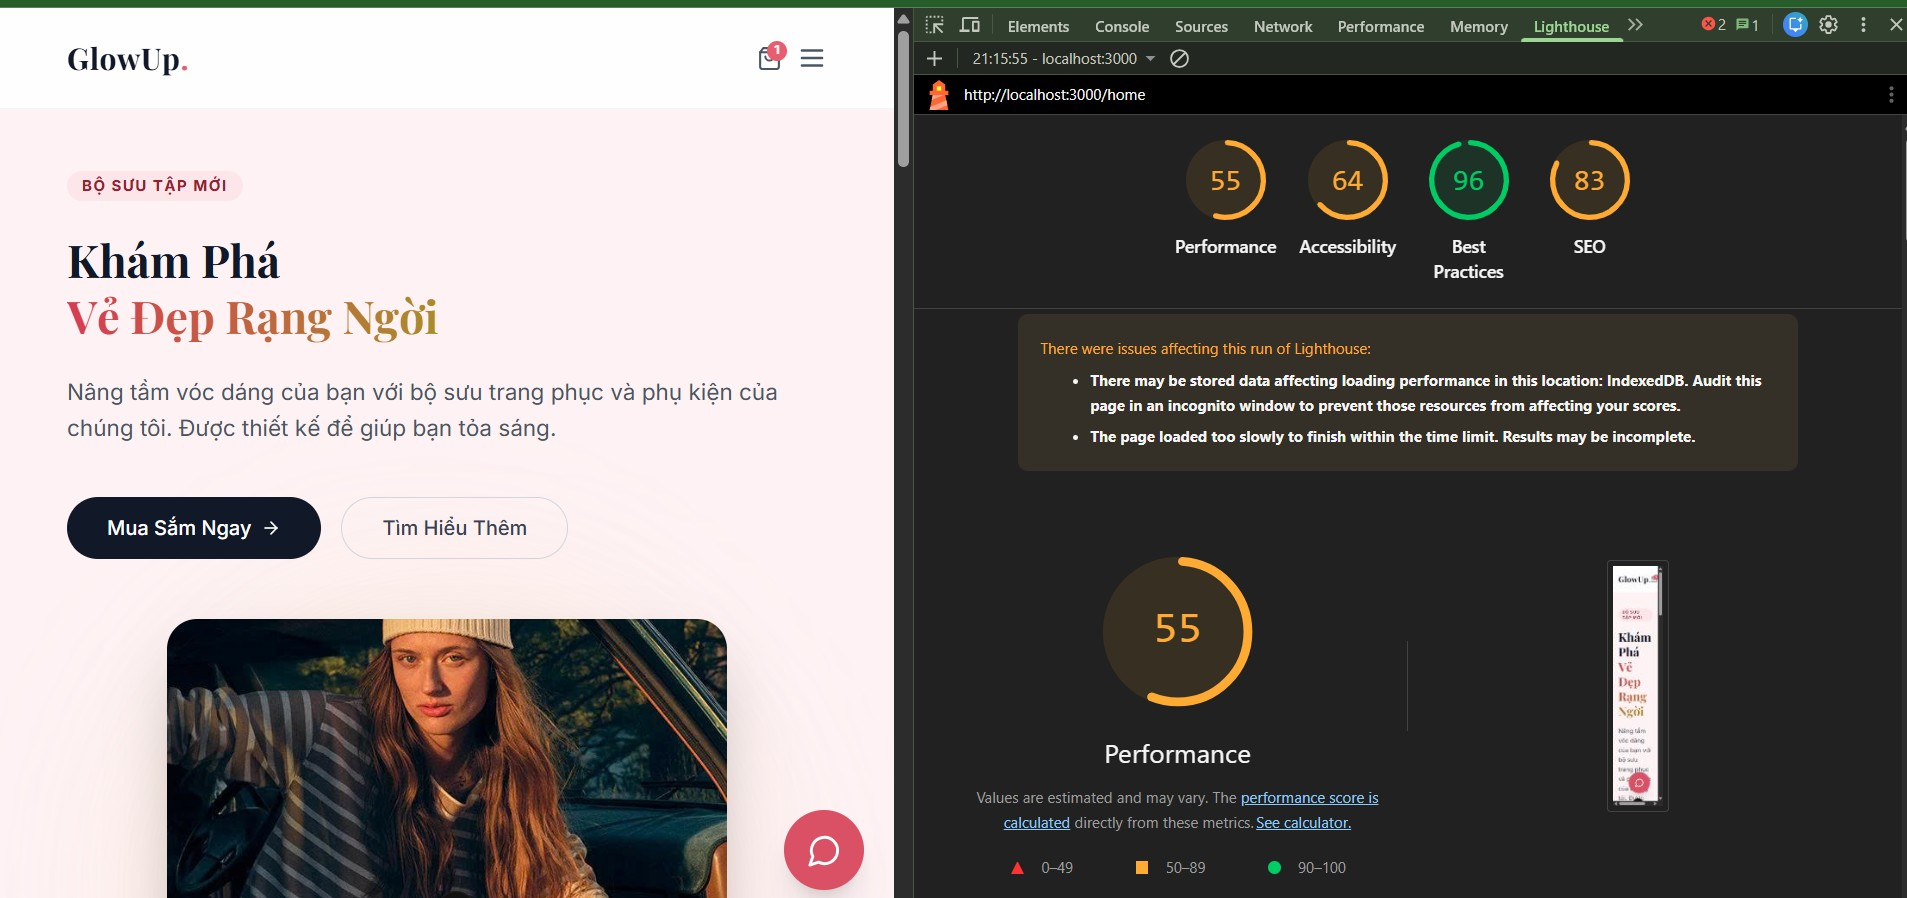
\includegraphics[width=\textwidth]{graphics/main/test/lighthouse_home.jpg}
    \caption{Kiểm thử hiệu năng trang chủ}
    \label{fig:lighthouse_home}
\end{figure}

\begin{figure}[H]
    \centering
    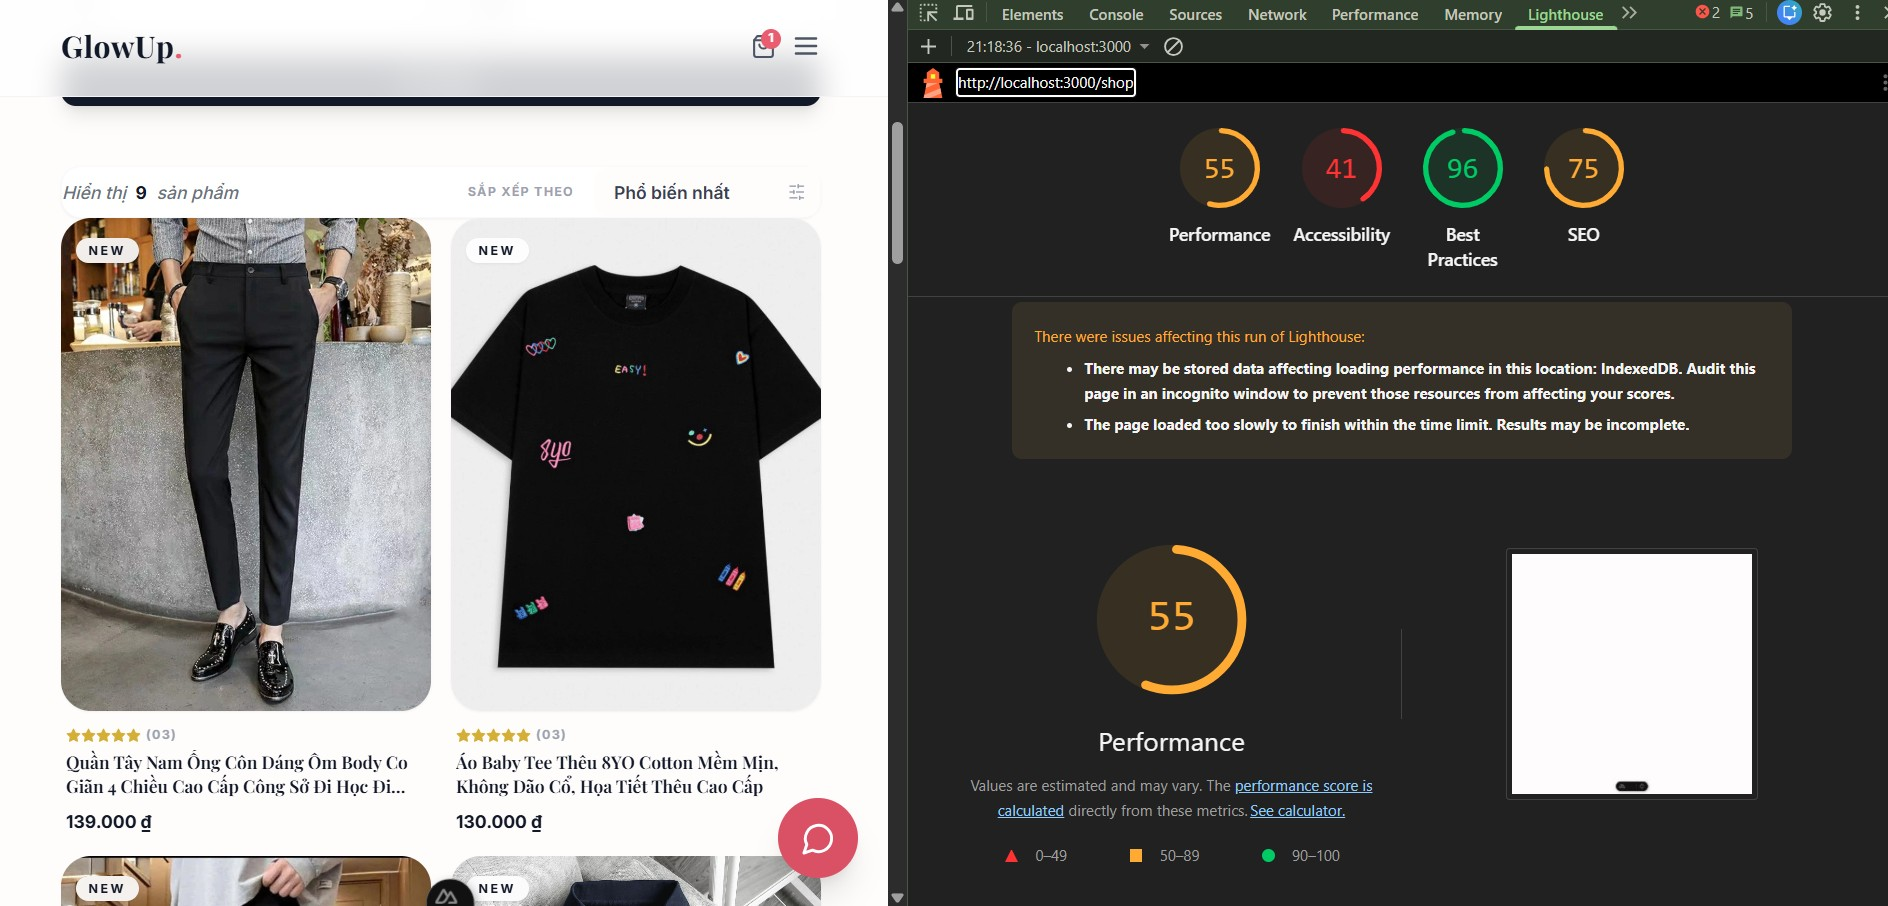
\includegraphics[width=\textwidth]{graphics/main/test/lighthouse_product.jpg}
    \caption{Kiểm thử hiệu năng trang danh sách sản phẩm}
    \label{fig:lighthouse_product}
\end{figure}

Các chỉ số đo lường trong kết quả Lighthouse:

\begin{itemize}
    \item \textbf{First Contentful Paint (FCP)}: Thời gian từ khi 
    người dùng mở trang cho đến khi trình duyệt hiển thị nội dung 
    đầu tiên (văn bản, ảnh, canvas...).
    
    \item \textbf{Largest Contentful Paint (LCP)}: Thời gian để 
    hiển thị phần tử nội dung lớn nhất trong vùng nhìn thấy, 
    thường là ảnh sản phẩm hoặc banner.
    
    \item \textbf{Total Blocking Time (TBT)}: Tổng thời gian 
    trình duyệt bị chặn bởi các tác vụ JavaScript dài (trên 50ms), 
    khiến người dùng không thể tương tác.
    
    \item \textbf{Cumulative Layout Shift (CLS)}: Mức độ thay đổi 
    bố cục khi trang tải, ví dụ văn bản bị đẩy xuống do ảnh 
    load chậm.
    
    \item \textbf{Speed Index}: Tốc độ trung bình mà nội dung 
    hiển thị trên màn hình trong quá trình tải trang, chỉ số 
    càng thấp càng tốt.
\end{itemize}
% ─────────────────────────────────────────
\subsubsection{Kiểm thử trên nhiều thiết bị}

Sử dụng extension Responsive Viewer trên Chrome để kiểm tra tính 
tương thích giao diện trên nhiều loại thiết bị:

\begin{itemize}
    \item \textbf{Điện thoại}: iPhone 14, iPhone 14 Plus, 
    iPhone SE, Samsung Galaxy S8, Galaxy S20
    \item \textbf{Máy tính bảng}: iPad Mini, iPad Air, iPad Pro
    \item \textbf{Máy tính}: Màn hình 1920$\times$1080px, 
    MacBook Pro 15 inch
\end{itemize}

\begin{figure}[H]
    \centering
    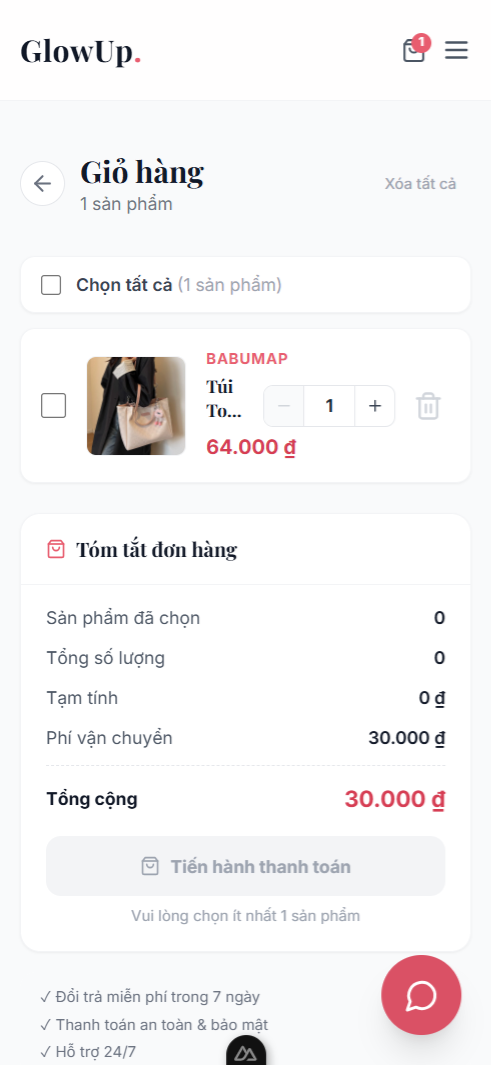
\includegraphics[width=\textwidth]{graphics/main/chapter4/responsive_cart_mobile.png}
    \caption{Kiểm thử giao diện trên thiết bị di động}
    \label{fig:responsive_mobile}
\end{figure}

\clearpage  % ← thêm dòng này

\begin{figure}[H]
    \centering
    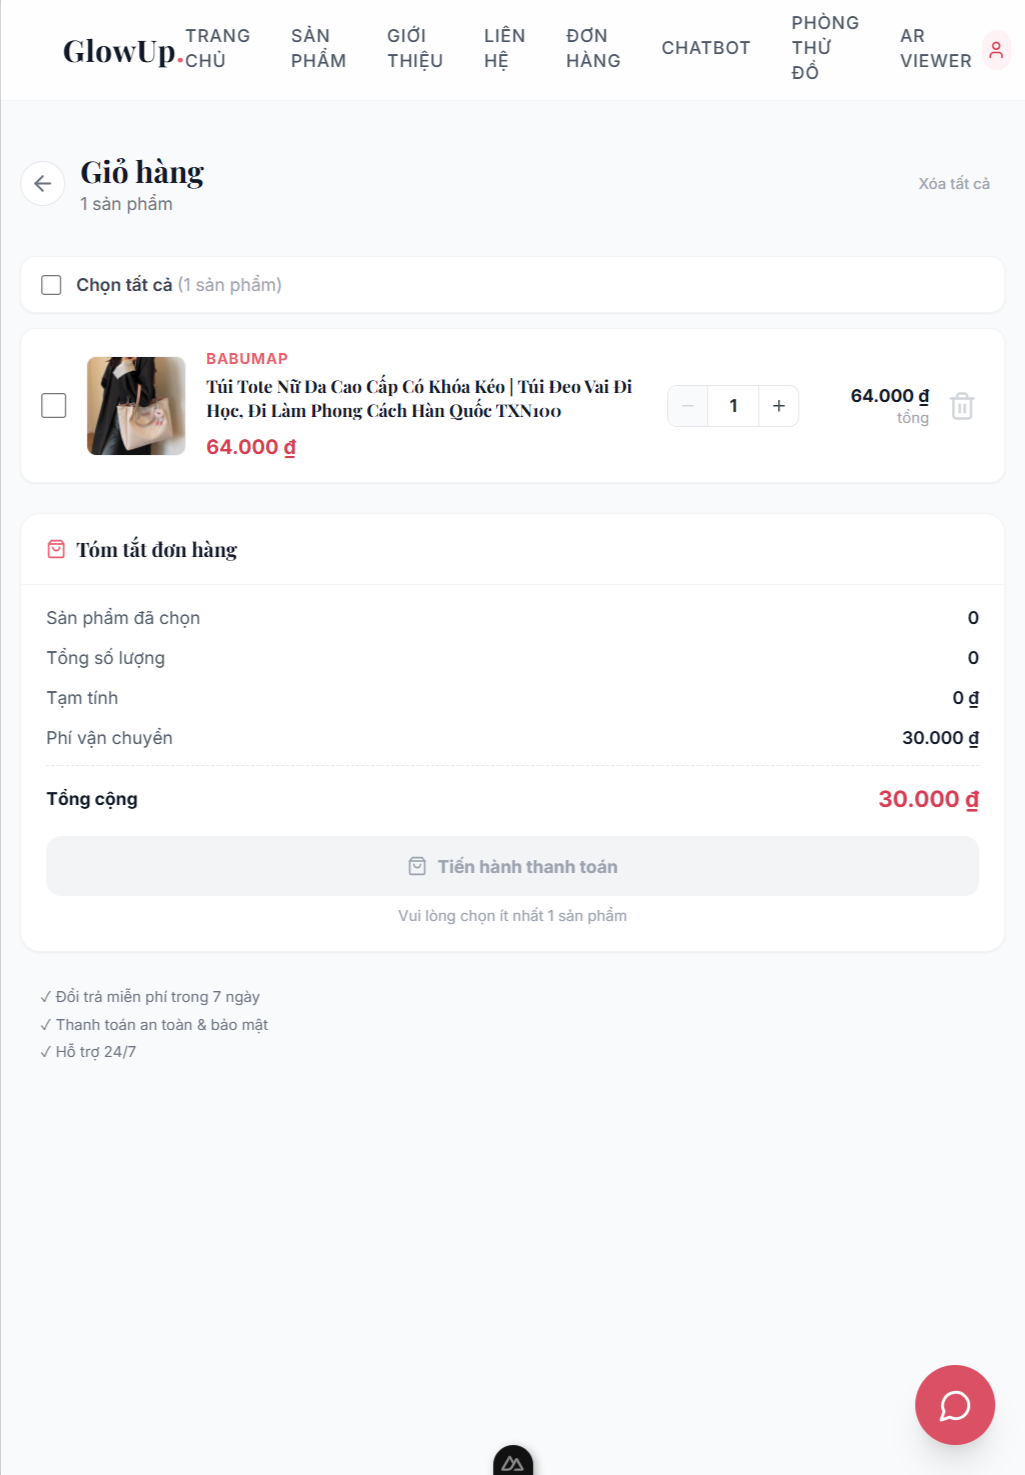
\includegraphics[width=\textwidth]{graphics/main/chapter4/responsive_cart_tablet.png}
    \caption{Kiểm thử giao diện trên máy tính bảng}
    \label{fig:responsive_tablet}
\end{figure}

Riêng chức năng \textbf{AR Try-On} được kiểm thử trực tiếp trên 
thiết bị thật do yêu cầu quyền truy cập camera thực tế, không 
thể giả lập qua Responsive Viewer.

% ─────────────────────────────────────────
\subsubsection{Kiểm thử trên nhiều trình duyệt}

Hệ thống được kiểm thử trên các trình duyệt phổ biến nhằm đảm 
bảo tính tương thích và hiển thị nhất quán.

\begin{table}[H]
\centering
\caption{Kết quả kiểm thử trên nhiều trình duyệt}
\label{tab:browser_test}
\begin{tabular}{|c|l|l|c|}
\hline
\textbf{STT} & \textbf{Trình duyệt} & \textbf{Chức năng kiểm tra} 
& \textbf{Kết quả} \\
\hline
1 & Google Chrome & Toàn bộ chức năng & Đạt \\
\hline
2 & Microsoft Edge & Giao diện, mua sắm, chatbot & Đạt \\
\hline
3 & Mozilla Firefox & Giao diện, mua sắm, chatbot & Đạt \\
\hline
\end{tabular}
\end{table}

\textit{Lưu ý: Chức năng AR Try-On sử dụng Snap Camera Kit hoạt 
động tốt nhất trên Google Chrome do yêu cầu hỗ trợ WebGL và 
quyền truy cập camera của trình duyệt.}